En este capítulo se muestran la planificación y presupuesto económico teórico del proyecto realizado teniendo en cuenta tanto los costes de personal como de equipos y gastos de tipo indirecto. Para ello se desglosará primero las distintas fases del proyecto con la carga en horas de cada uno, y posteriormente se calcularán los costes totales.

\section{Fases del proyecto}

Conocer las fases del proyecto es necesario para estimar los costes económicos asociados a cada fase.
A continuación, se describen las fases en las que se ha desarollado el proyecto.
Además, en la Figura~\ref{fig:gantt} se muestra de forma visual la planificación del proyecto en base a un diagrama de Gantt.

\begin{figure}[H]
    \centering
    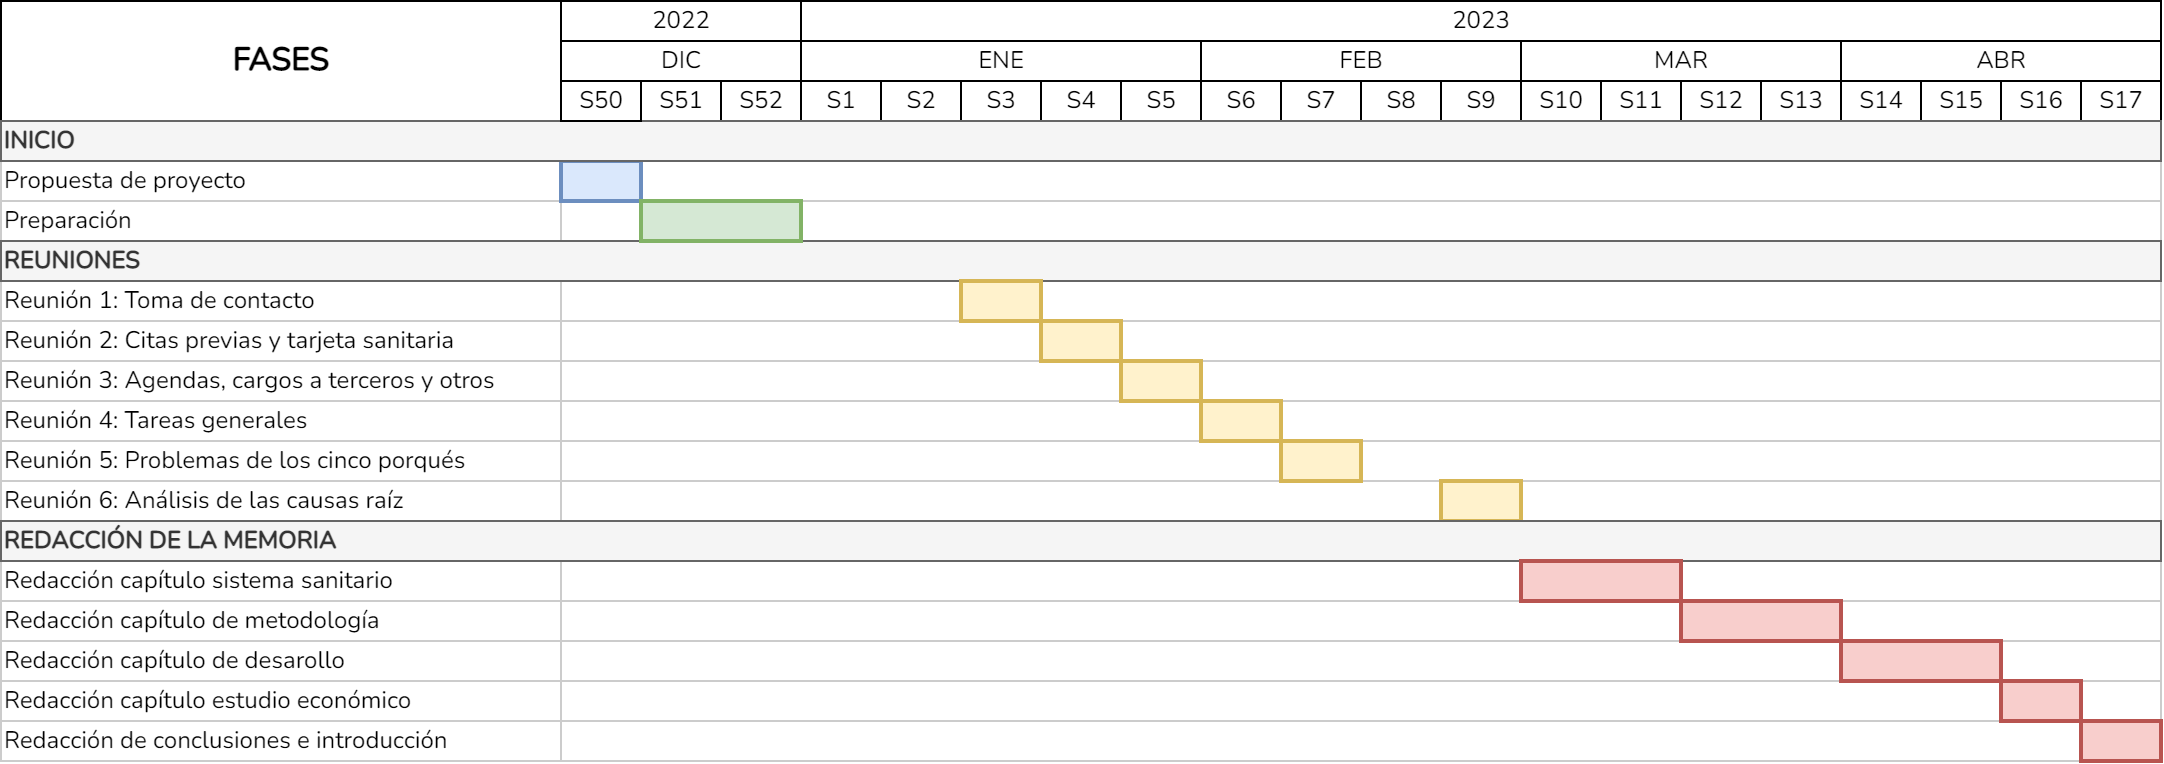
\includegraphics[width=\textwidth]{img/gantt-diagram.png}
    \caption{Diagrama de Gantt del proyecto}
    \label{fig:gantt}
\end{figure}

\subsection{Propuesta}

El proyecto comienza con la propuesta por parte de la Subdirección de Gestión del Área de Salud Valladolid Oeste. En esta fase se exponen los objetivos que se quieren alcanzar además de propuestas sobre la metodología a seguir.

\subsection{Preparación}

Antes de formar al grupo de trabajo del centro de salud, es necesario documentarse en la aplicación de técnicas lean y de mejora continua en entornos de oficina y sanitarios. Además, en esta fase se preparó una página web en \Gls{sharepoint} en donde ir actualizando semanalmente todo el contenido del proyecto.

\subsection{Reuniones de grupo}

Para conocer en detalle la sección administrativa del centro se organizaron reuniones semanales con un grupo pequeño de trabajadores a modo de muestra que conocieran bien su puesto de trabajo.
Se realizaron un total de seis reuniones que se pueden separar en dos fases.
Por un parte las cuatro primeras reuniones se centraron en recoger información de todas las tareas administrativas que se realizan en los puestos administrativos de cara a definir un estándar y, por otras parte, las dos últimas reuniones se centraron en obtener un listado de problemas su posterior análisis de las causas raíz.

\subsubsection{Reunión 1: Toma de contacto}

En esta primera reunión asistieron los dos subdirectores de gestión. Fue una presentación corta en la que se explicó al grupo de trabajo la necesidad de realizar una estandarización de las tareas administrativas de la sección del centro con el fin de analizar las cargas de trabajo reales. Además, se propuso el análisis mediante la técnica de los cinco porqués las causas raíz de los problemas administrativos.

\subsubsection{Reunión 2: Citas previas y tarjeta sanitaria}

Dado que la gestión de citas principales, y consecuentemente más tiempo consumen, fue el primer proceso que se trató. Se explicó con detalle los distintos tipos de citas: médico de familia, enfermera, trabajador social, ginecología, extracción y radiología. Además de explicar el proceso, se entregó una copia a modo de ejemplo de los volantes de extracciones y de radiología en los cuales el facultativo especifica qué pruebas concretas se deben de realizar al paciente.

\subsubsection{Reunión 3: Agendas, cargos a terceros, reclamaciones y absentismo}

En esta reunión se trataron los procesos de gestión de agendas, la tramitación de cargos a terceros, reclamaciones y las solicitudes de permisos retribuidos.

\subsubsection{Reunión 4: Tareas generales}

En esta última reunión sobre la estandarización se desarrollaron por parte del personal otras tareas generales que no pertenecen a ninguno de los procesos principales.

\subsubsection{Reunión 5: Listado de problemas para los cinco porqués}

Presentación y explicación de la herramienta de los cinco porqués.
Se realizó un ``brainstorming'' para obtener todos los problemas que existen en la sección administrativas.
Posteriormente se filtraron para valorar los que más impacto tenían en el rendimiento del equipo.

\subsubsection{Reunión 6: Análisis de las causas raíz y propuestas de mejora}

En esta última reunión se fueron comentando cada uno de los problemas listados en la anterior reunión a la vez que se aplicaba la ténica de los cinco porqués.
Una vez obtenidos las causas de cada problema, se propusieron posibles soluciones a cada una de las problemáticas.
Finalmente, se discutió la viabilidad de cada una.

\subsection{Redacción del informe}

Finalmente, tras recoger todos los datos necesarios se procede a analizar los resultados y a redactar la memoria del trabajo. 

\section{Estimación de costes}

En este apartado se llevará a cabo el desglose de los distintos tipos de costes que conlleva el proyecto. Esto incluye los costes del personal implicado, costes de amortización de los equipos y costes indirectos.

\subsection{Costes de personal}

Los costes de personal corresponden a todas las personas implicadas en el proyecto que han dedicado parte de su jornada laboral al mismo: subdirectores y administrativos principalmente.
En la Tabla~\ref{tab:horas-trabajadas} se muestra el reparto de horas trabajadas por cada grupo de personal y por fase de proyecto.
Cabe destacar que en la columna de administrativos se ha tenido en cuenta las horas dedicadas por los cuatro trabajadores de la sección administrativa del centro de salud.

\begin{table}[H]
    \centering
    \begin{tabular}{llll}
        \toprule
        Fases               & Ingeniero & Subdirectores & Administrativos \\
        \midrule
        Propuesta           & 8         & 1             & 0               \\
        Preparación         & 32        & 0             & 0               \\
        Reuniones de grupo  & 48        & 12            & 48              \\
        Elaboración informe & 212       & 0             & 0               \\
        \midrule
        Total               & 300       & 13            & 48              \\
        \bottomrule
    \end{tabular}
    \caption{Desglose de horas dedicadas por personal y fase}
    \label{tab:horas-trabajadas}
\end{table}

Una vez obtenida la dedicación en horas se procede a calcular los costes de personal. Para ello se utilizará la tabla de retribuciones salariales de la Gerencia Regional de Salud correspondiente al año vigente, 2023, para calcular el coste por hora trabajada. Es importante, tener en cuenta que el número total de horas trabajadas por año en el Sacyl es de 1645 horas para turnos fijos diurnos.

\begin{itemize}
    \item Ingeniero: 23.13 euros/hora
    \item Subdirector de Gestión: 34.40 euros/hora
    \item Administrativo: 11.78 euros/hora
\end{itemize}

Finalmente, en la Tabla~\ref{tab:coste-horas} se muestran los costes totales de personal para todo el proyecto.

\begin{table}[H]
    \centering
    \begin{tabular}{llll}
        \toprule
        Fases               & Ingeniero & Subdirectores & Administrativos \\
        \midrule
        Propuesta           & 185.04    & 34.40         & 0               \\
        Preparación         & 740.16    & 0             & 0               \\
        Reuniones de grupo  & 1110.24   & 277.56        & 565.44          \\
        Elaboración informe & 4093.56   & 0             & 0               \\
        \midrule
        Total               & 6939      & 447.2         & 565.44          \\
        \bottomrule
    \end{tabular}
    \caption{Coste en euros de personal por fase y posición}
    \label{tab:coste-horas}
\end{table}

\subsection{Costes de amortización}

En este apartado se han calculado los costes de las amortizaciones de los equipos utilizados en el proyecto.
La amortización es la pérdida de valor que los bienes del inmovilizado de la empresa sufren a medida que se van usando, porque se producen avances con la investigación que hacen que se vayan quedando anticuados o por el mero transcurso del tiempo.
En este caso fue necesario el uso de un ordenador junto con un conjunto de periféricos.
También se incluyen las licencias de los distintos programas informáticos utilizados.

La amortización de estos equipos se ha calculado considerando una vida útil de cinco años tal y como se muestra en la Tabla~\ref{tab:coste-equipos}.

\begin{table}[H]
    \centering
    \begin{tabular}{lll}
        \toprule
        Equipo              & Precio  & Amortización \\
        \midrule
        Ordenador HP        & 783.34  & 156.67       \\
        Licencia Windows 10 & 108.23  & 21.65        \\
        Licencia Office 365 & 127.12  & 25.42        \\
        Impresora Kyocera   & 97.23   & 19.45        \\
        \midrule
        Total               & 1115.92 & 223.19       \\
        \bottomrule
    \end{tabular}
    \caption{Amortización anual en euros de los equipos utilizados}
    \label{tab:coste-equipos}
\end{table}

\subsection{Costes indirectos}

El coste indirecto es aquel que afecta al proyecto pero que no puede imputarse a ninguna de las fases o etapas del mismo.
En este caso se hacen referencia a los consumos de electricidad, conexión a internet, alquiler, etc.
En la Tabla~\ref{tab:coste-indirecto} se resumen los costes indirectos del proyecto.

\begin{table}[H]
    \centering
    \begin{tabular}{ll}
        \toprule
        Coste        & Coste \\
        \midrule
        Alquiler     & 375   \\
        Mobiliario   & 55    \\
        Electricidad & 35    \\
        Internet     & 50    \\
        Transporte   & 55    \\
        \midrule
        TOTAL        & 570   \\
        \bottomrule
    \end{tabular}
    \caption{Coste indirecto en euros del proyecto}
    \label{tab:coste-indirecto}
\end{table}

\subsection{Costes totales}

La estimación del coste total de trabajo de fin de máster se obtiene de la suma de los distintos costes totales de cada una de las partidas definidas en los apartados anteriores.
En la Tabla~\ref{tab:coste-total} se reflejan todos los costes y su peso sobre el total.

\begin{table}[H]
    \centering
    \begin{tabular}{lll}
        \toprule
        Concepto          & Coste   & Porcentaje \\
        \midrule
        Personal          & 7951.64 & 91\%       \\
        Amortización      & 223.19  & 3\%        \\
        Costes indirectos & 570     & 6\%        \\
        \midrule
        TOTAL             & 8744.83 & 100\%      \\
        \bottomrule
    \end{tabular}
    \caption{Coste total en euros del proyecto}
    \label{tab:coste-total}
\end{table}

A estos costes habría que sumar impuestos indirectos como el IVA y el margen comercial de beneficio.